\chapter{Sana System}
Sana System is belived to be an Iranian malware targeting Iranian cellphones. The virus logs the user phone number and sends it to a remote server. In addition the virus also reads every incoming SMS messages and sends them to the aforementioned server, this could be used to steal sensitive information like 2FA codes. After doing some online research we discovered an article were it is mentioned that a similar virus with the same app name is installed from a fake minister of justice site where the user also insert his bank account information under the pretext of showing juridical documents and, after infecting the user phone, sends malicious links to other phone contacts to spread the virus. We are certain that the viruses are different since the one we analyzed does not have any permission to access contacts info and write messages, however, due to the stunning similarity in presentation and SMS handling, we decided to point out this thing. This could be indicate them being part of the same phishing campaign originating from the same group.

\section{VirusTotal}
We started by feeding the APK to the VirusTotal tool:
\begin{figure}[H]
\centering
    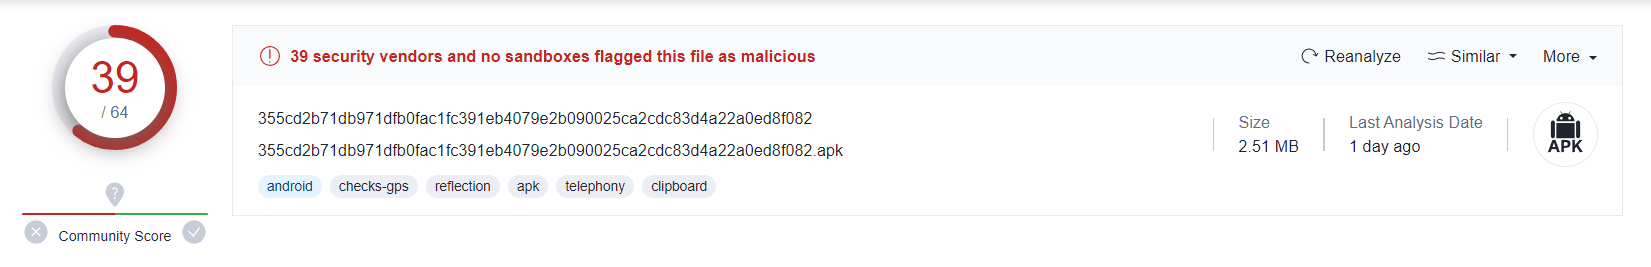
\includegraphics[width=1\textwidth]{./images/screenshot/SanaSystem/ReviewSanaSystem.png}
    \caption{Review score of Sana System}
    \label{fig:SanaReview}
\end{figure}

As it can be seen the score of 39 out of 64 indicate a very high chance of being a virus. In general many anti-malwares, like Avast or Kaspersky, flag this software as malicious as it can be seen in Fig. \ref{fig:SanaDetection}.

\begin{figure}[h!]
\centering
    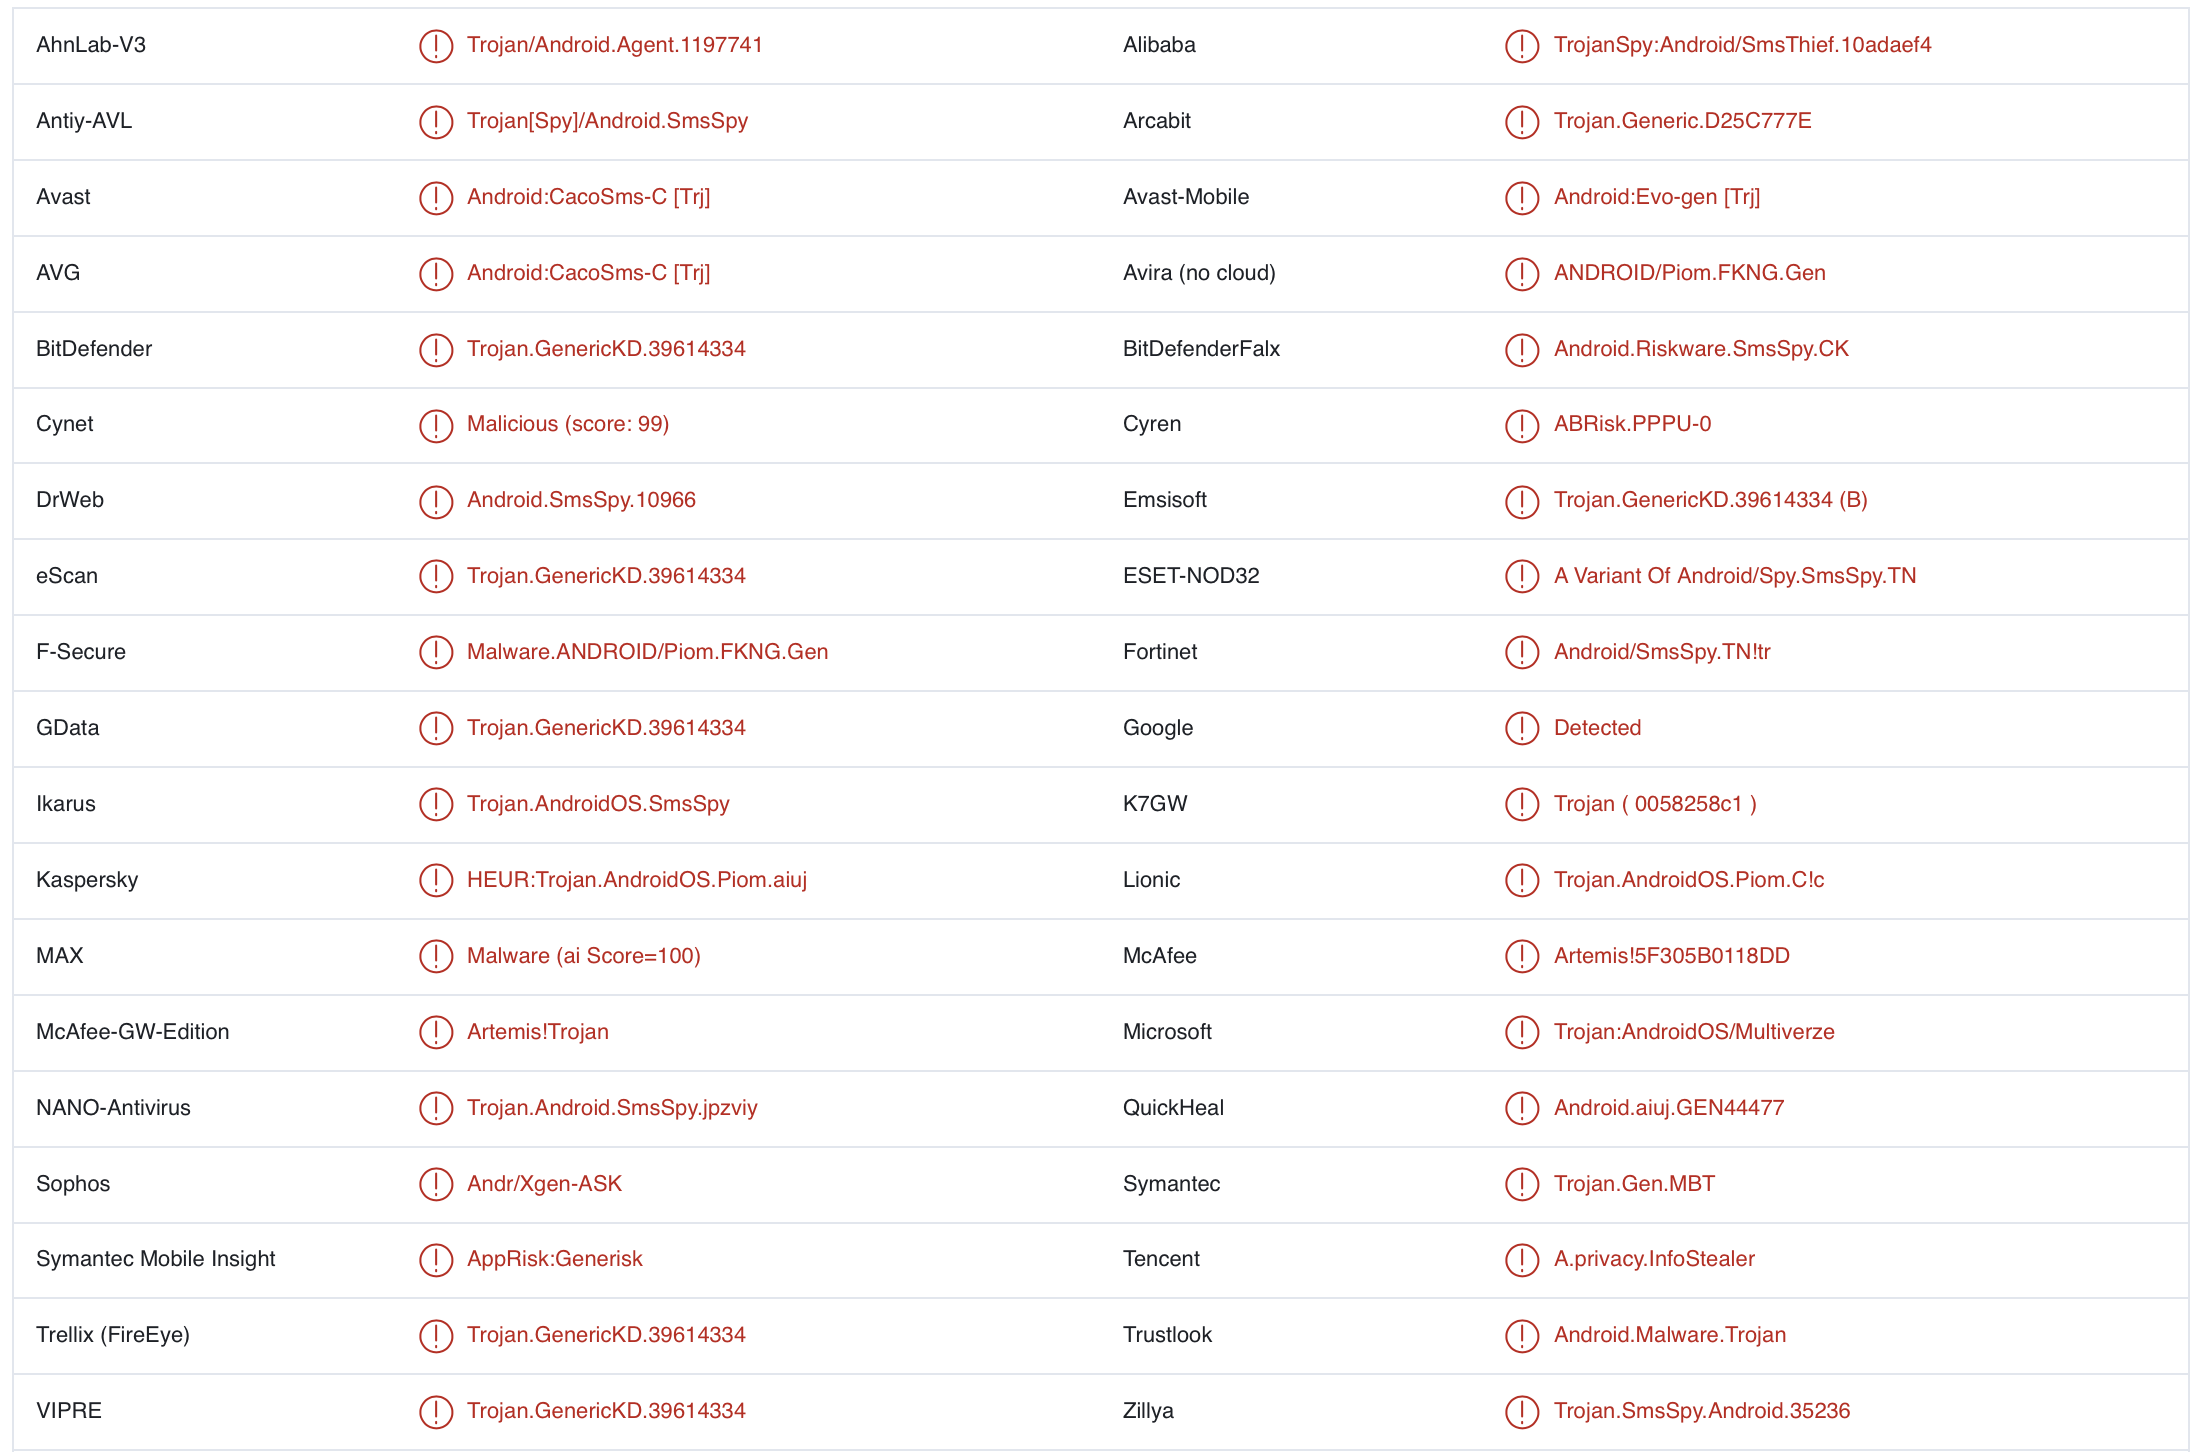
\includegraphics[width=1\textwidth]{./images/screenshot/SanaSystem/Detection.png}
    \caption{Anti-malware detection}
    \label{fig:SanaDetection}
\end{figure}

In general the malware is identify as a trojan/smsspy this is also indicated by the permission required by the app.
\begin{figure}
\centering
    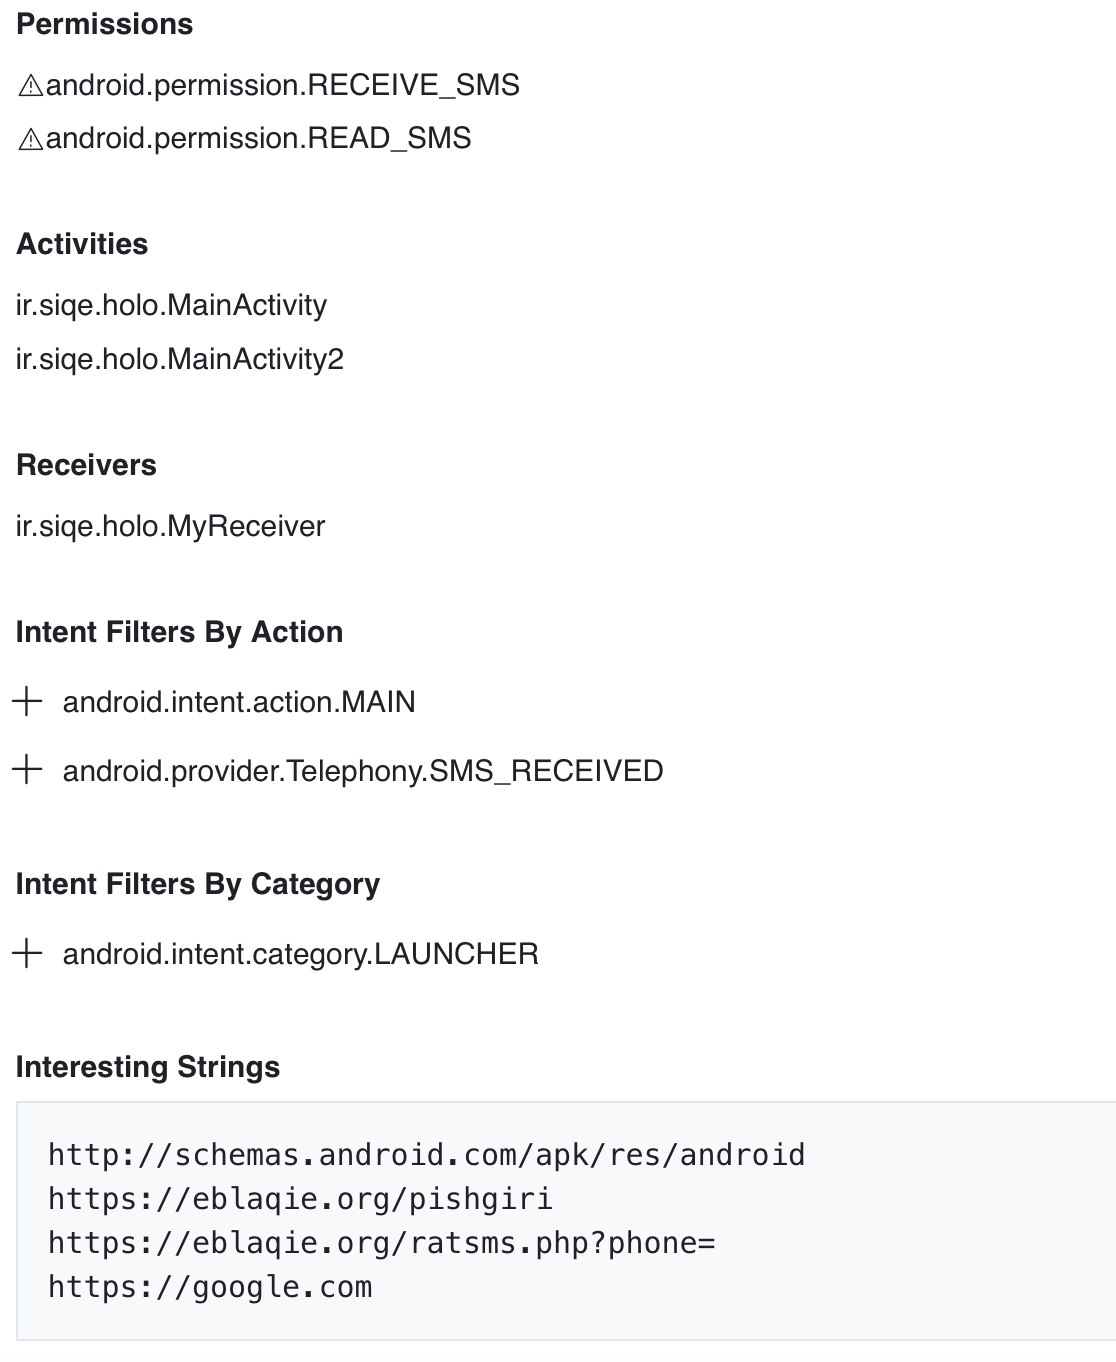
\includegraphics[scale=0.5]{./images/screenshot/SanaSystem/Details.png}
    \caption{Details highlighted by virus total}
    \label{fig:SanaDetails}
\end{figure}
As shown in Fig. \ref{fig:SanaDetails} the app request permission to receive SMS and read them, in addition it requires permission to access network state and create internet connection. This can be seen in the manifest Fig \ref{fig:SanaManifest}.
\begin{figure}[h!]
\centering
    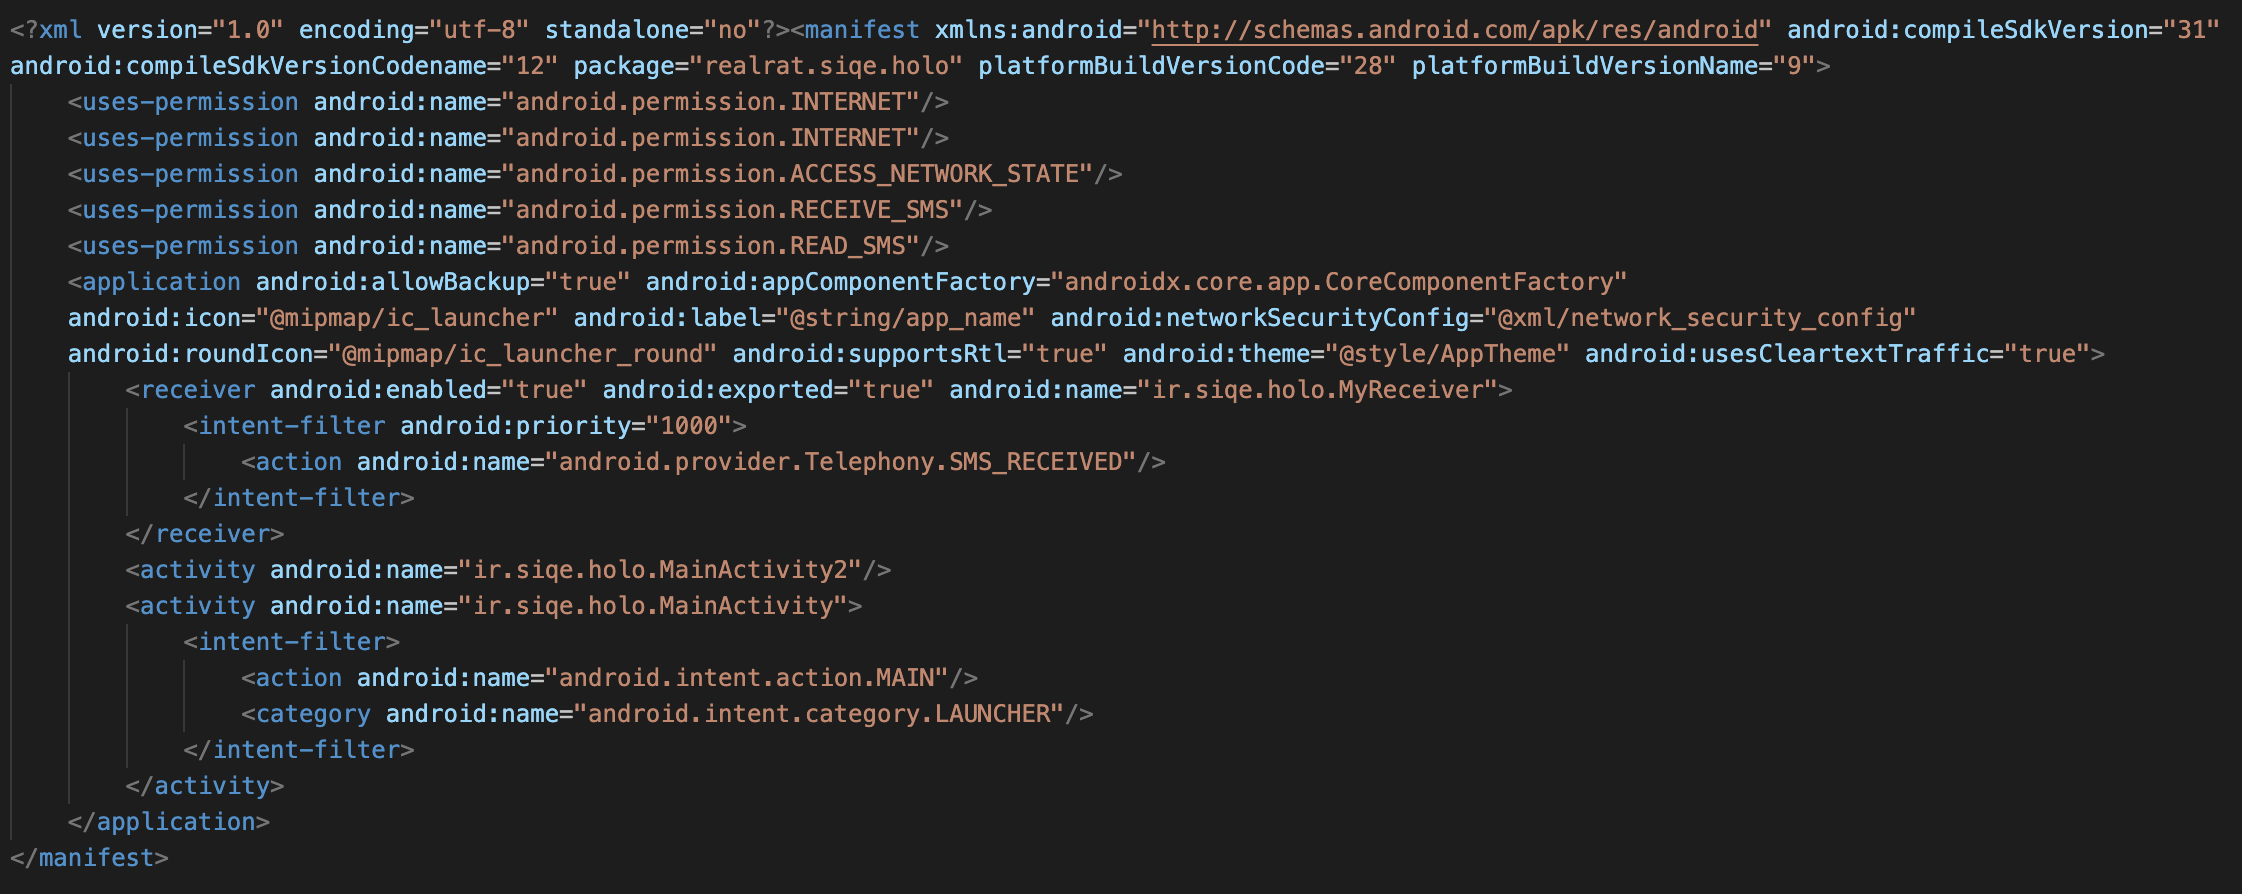
\includegraphics[width=1\textwidth]{./images/screenshot/SanaSystem/Manifest.png}
    \caption{App manifest}
    \label{fig:SanaManifest}
\end{figure}

Virus total also signaled the presence of some interesting string such as: "\emph{https://eblaqie.org/pishgiri}" and "\emph{https://eblaqie.org/ratsms.php?phone=}". In particular the second one, as we shall see in the next pages, is used to perform a GET operation to a server where the phone number and relative SMS messages are logged.

In addition Virus Total shows us the detected contacted domains, where eblaqie.org is present and is the only one reached by the app Fig. \ref{fig:ContactedDom}.
\begin{figure}
\centering
    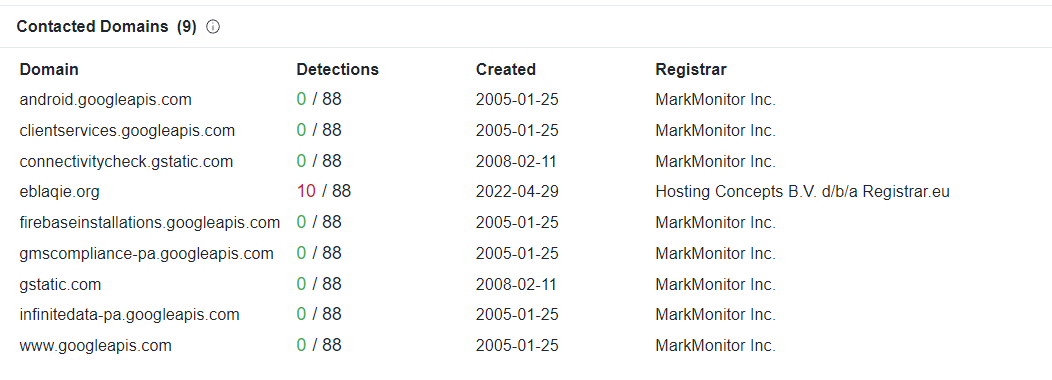
\includegraphics[width=1\textwidth]{./images/screenshot/SanaSystem/Domains.png}
    \caption{Contacted domains}
    \label{fig:ContactedDom}
\end{figure}


\section{MobSF}
We then proceed by feeding the APK to MobSF and got the header in Fig. \ref{fig:mobsfHeader}, due to the exhaustiveness of Virus Total answer we decided not to show the almost identical result of the static analysis. 

\begin{figure}[h!]
\centering
    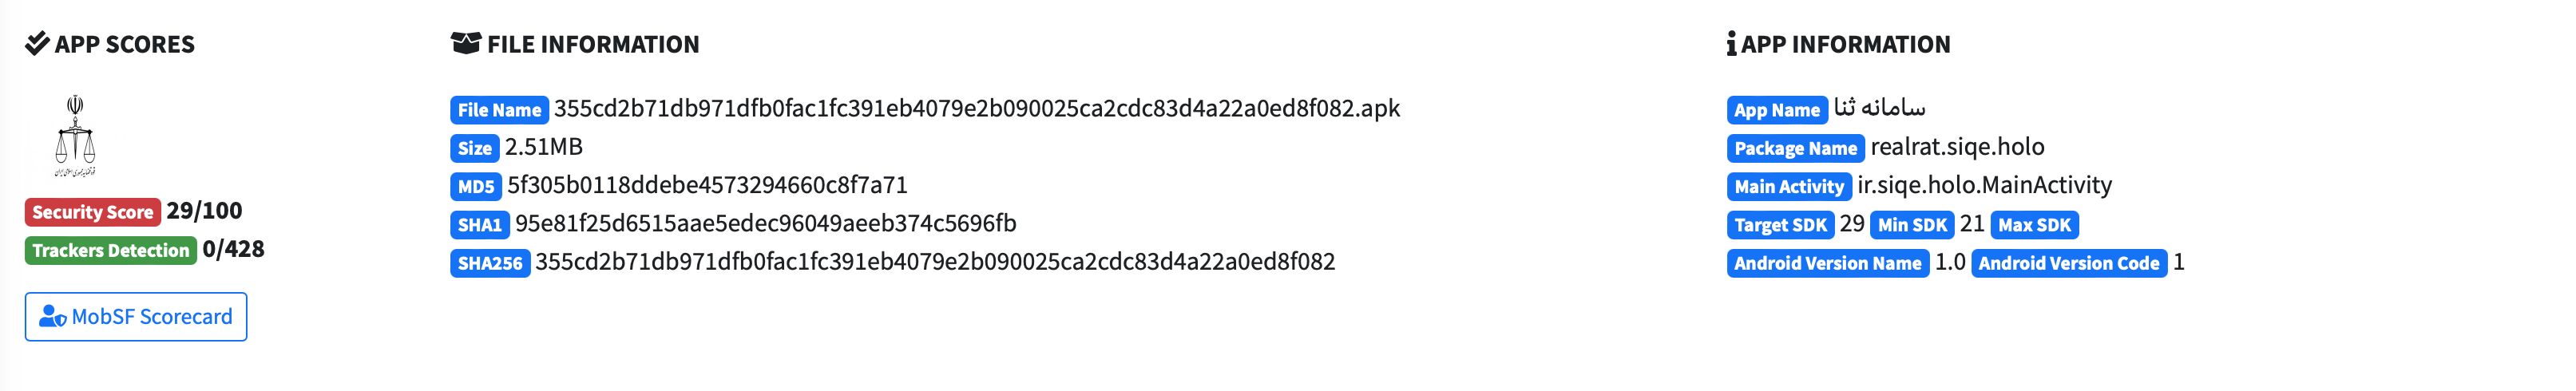
\includegraphics[width=1\textwidth]{./images/screenshot/SanaSystem/HeaderMobSF.png}
    \caption{Header of MobSF}
    \label{fig:mobsfHeader}
\end{figure}

Another thing to point out is that eblaqie.org is signaled by Maltrail, a publicly available domain blacklist, as a malicious domain and it is not to be trusted (Fig. \ref{fig:MalTrail}). 

\begin{figure}[h!]
\centering
    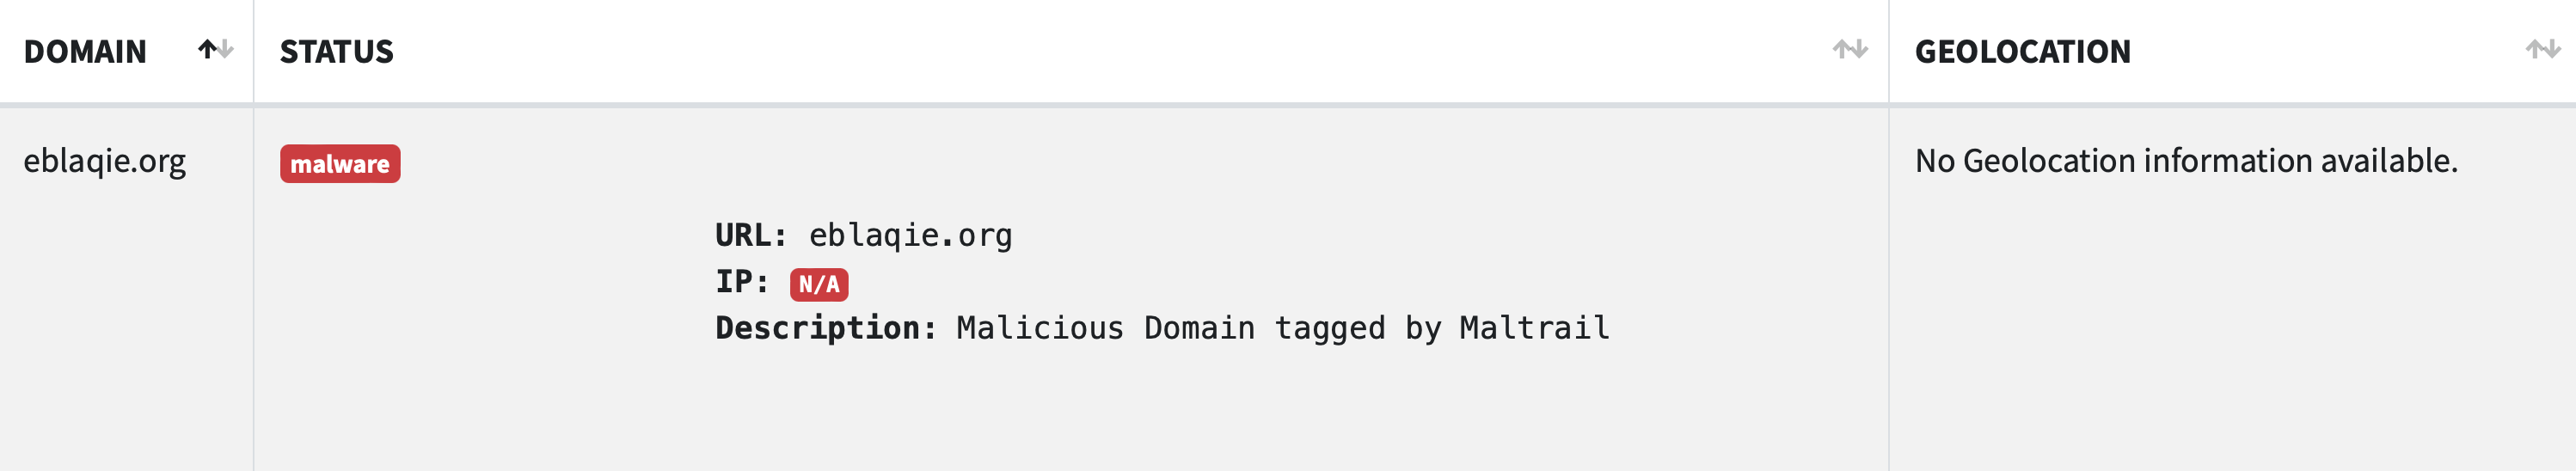
\includegraphics[width=1\textwidth]{./images/screenshot/SanaSystem/eblaqieDomain.png}
    \caption{Tag of eblaqie.org}
    \label{fig:MalTrail}
\end{figure}

\section{Code Analysis}
We start this code analysis by looking into the code structure shown in Fig. \ref{fig:SanaPackage} and specifically into ir.siqe.holo package highlighted by MobSF in Fig. \ref{fig:mobsfHeader} where the main activity is placed, Virus total (Fig. \ref{fig:SanaDetails}) also confirms MainActivity to be the de facto main of the software. The others package are libraries and there is no evidence of them being tampered with.

\begin{figure}[h!]
\centering
    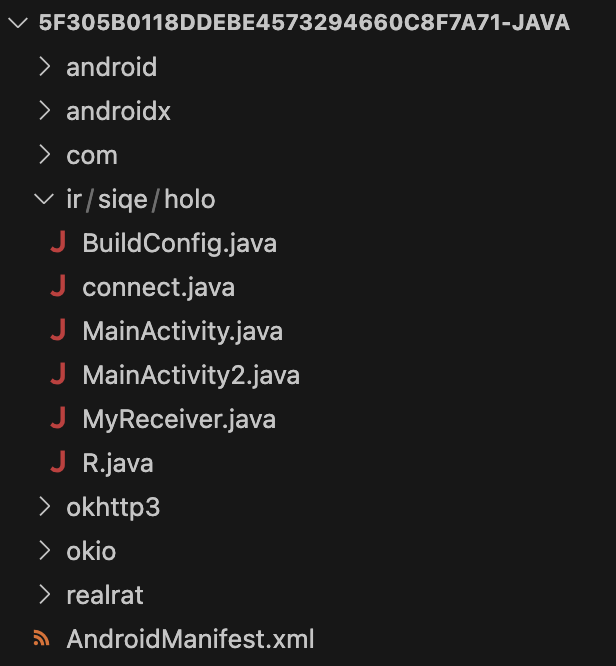
\includegraphics[width=0.6\textwidth]{./images/screenshot/SanaSystem/Package.png}
    \caption{Package organization}
    \label{fig:SanaPackage}
\end{figure}
\newpage

\subsection{MainActivity}
MainActivity extends AppCompatActivity that allow to use the newer feature of android on older devices and, given the fact that the minimum SDK required to run the software is Android 5.0, allows the use of this app on devices that no longer receive security update. After the activity is launched onCreate method is called, Bundle is typically used for passing data between various Android activities. 
After setting the screen presented to the user, the app waits for a text input in the form of a number. Then when the user clicks on the button with id "go" there is a check with a regular expression, for matching an iranian telephone number (+98 as prefix), if the number not matches it displays a small popup (Toast) that says \textit{"The mobile number is not valid"} and does nothing else, otherwise ask for permission to receive SMS and, if given, calls the method \textit{connect} to log to a remote server the inputted number with a string identifying the new entry, then a new activity starts and the code stream goes to MainActivity2.

\begin{figure}[h!]
\centering
    \includegraphics[width=1\textwidth]{./images/screenshot/SanaSystem/MainActivity.png}
    \caption{MainActivity}
    \label{fig:MalTrail}
\end{figure}
\newpage


